% Source: Wald GR, physical PDF p. 170
%         (printed p. 157).
% Coverage: Figure 6.12, another representation of the Figure 6.11 spacetime.
% Figures/tables/footnotes: Figure 6.12; no tables or footnotes.
% Status: source-reviewed and compile-clean.
% Uncertainties: none.
\begingroup
\renewcommand{\thefigure}{6.12}
\begin{figure}[htbp]
\centering
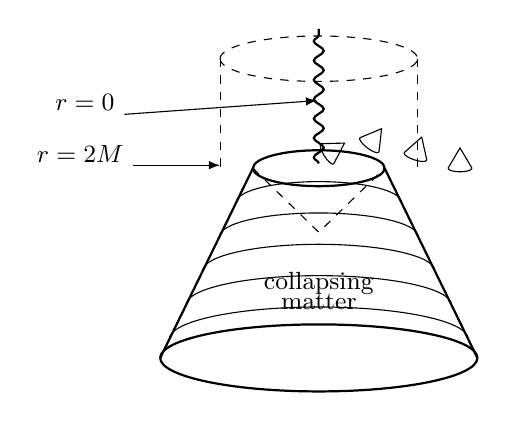
\begin{tikzpicture}[scale=.76,>=latex,font=\small]
  \draw[dashed] (-1.65,2.65) arc[start angle=180,end angle=360,x radius=1.65,y radius=.38];
  \draw[dashed] (-1.65,2.65) arc[start angle=180,end angle=0,x radius=1.65,y radius=.38];
  \draw[dashed] (-1.65,2.65) -- (-1.65,.75);
  \draw[dashed] (1.65,2.65) -- (1.65,.75);
  \draw[thick] (-2.65,-2.35) arc[start angle=180,end angle=360,x radius=2.65,y radius=.56];
  \draw[thick] (-2.65,-2.35) arc[start angle=180,end angle=0,x radius=2.65,y radius=.56];
  \draw[thick] (-2.65,-2.35) -- (-1.10,.82);
  \draw[thick] (2.65,-2.35) -- (1.10,.82);
  \draw[thick] (-1.10,.82) arc[start angle=180,end angle=360,x radius=1.10,y radius=.30];
  \draw[thick] (-1.10,.82) arc[start angle=180,end angle=0,x radius=1.10,y radius=.30];
  \foreach \t in {.1,.28,.46,.64,.82} {
    \draw[thin] ({-2.65+1.55*\t},{-2.35+3.17*\t}) arc[start angle=180,end angle=0,
      x radius={2.65-1.55*\t},y radius={.56-.26*\t}];
  }
  \draw[thick,decorate,decoration={snake,amplitude=1.8pt,segment length=7pt}]
    (0,.90) -- (0,3.15);
  \foreach \x/\y/\a in {.43/1.24/-58,1.05/1.48/-37,1.72/1.34/-18,2.36/1.16/0} {
    \begin{scope}[shift={(\x,\y)},rotate=\a]
      \draw[thin] (-.20,-.34) -- (0,0) -- (.20,-.34);
      \draw[thin] (-.20,-.34) arc[start angle=180,end angle=360,x radius=.20,y radius=.06];
    \end{scope}
  }
  \draw[dashed] (-1.10,.82) -- (0,-.25) -- (1.10,.82);
  \node at (0,-1.10) {collapsing};
  \node at (0,-1.42) {matter};
  \draw[->] (-3.25,1.72) -- (-.03,1.95);
  \node[left] at (-3.25,1.92) {\(r=0\)};
  \draw[->] (-3.10,.87) -- (-1.65,.87);
  \node[left] at (-3.10,1.06) {\(r=2M\)};
\end{tikzpicture}
\caption{Another representation of the spacetime of Figure~\ref{fig:6.11}.
Here, one of the two suppressed spatial dimensions is restored, so each of the
circles shown on the collapsing body corresponds to the 2-sphere surface of the
body at an instant of time. However, the light cones no longer are represented by
\(45^\circ\) lines. Indeed, the spacelike nature of the singularity and the
inevitable capture by the singularity of any particle or light ray in the region
\(r<2M\) is illustrated here by the tipping over of the future light cones in the
strong field region.}
\label{fig:6.12}
\end{figure}
\endgroup
